As compute capabilities continue to outpace I/O capacity on supercomputers, \textit{in situ} processing is an increasingly important solution to enable analysis of large-scale simulation data~\cite{bauer2016situ}.
%
In situ processing involves coupling with the simulation code and operating on the full spatiotemporal resolution of the data in memory. 
%
However, in situ analysis tasks operate in constrained environments and are afforded limited execution time and memory.
%
Consequently, analysis tasks must scale effectively since simulations execute across hundreds of compute nodes~(CNs).
%
In this paper, we investigate the performance of in situ data reduction via Lagrangian analysis to enable exploratory time-varying vector field analysis.
%
\begin{figure}[!t]
\centering
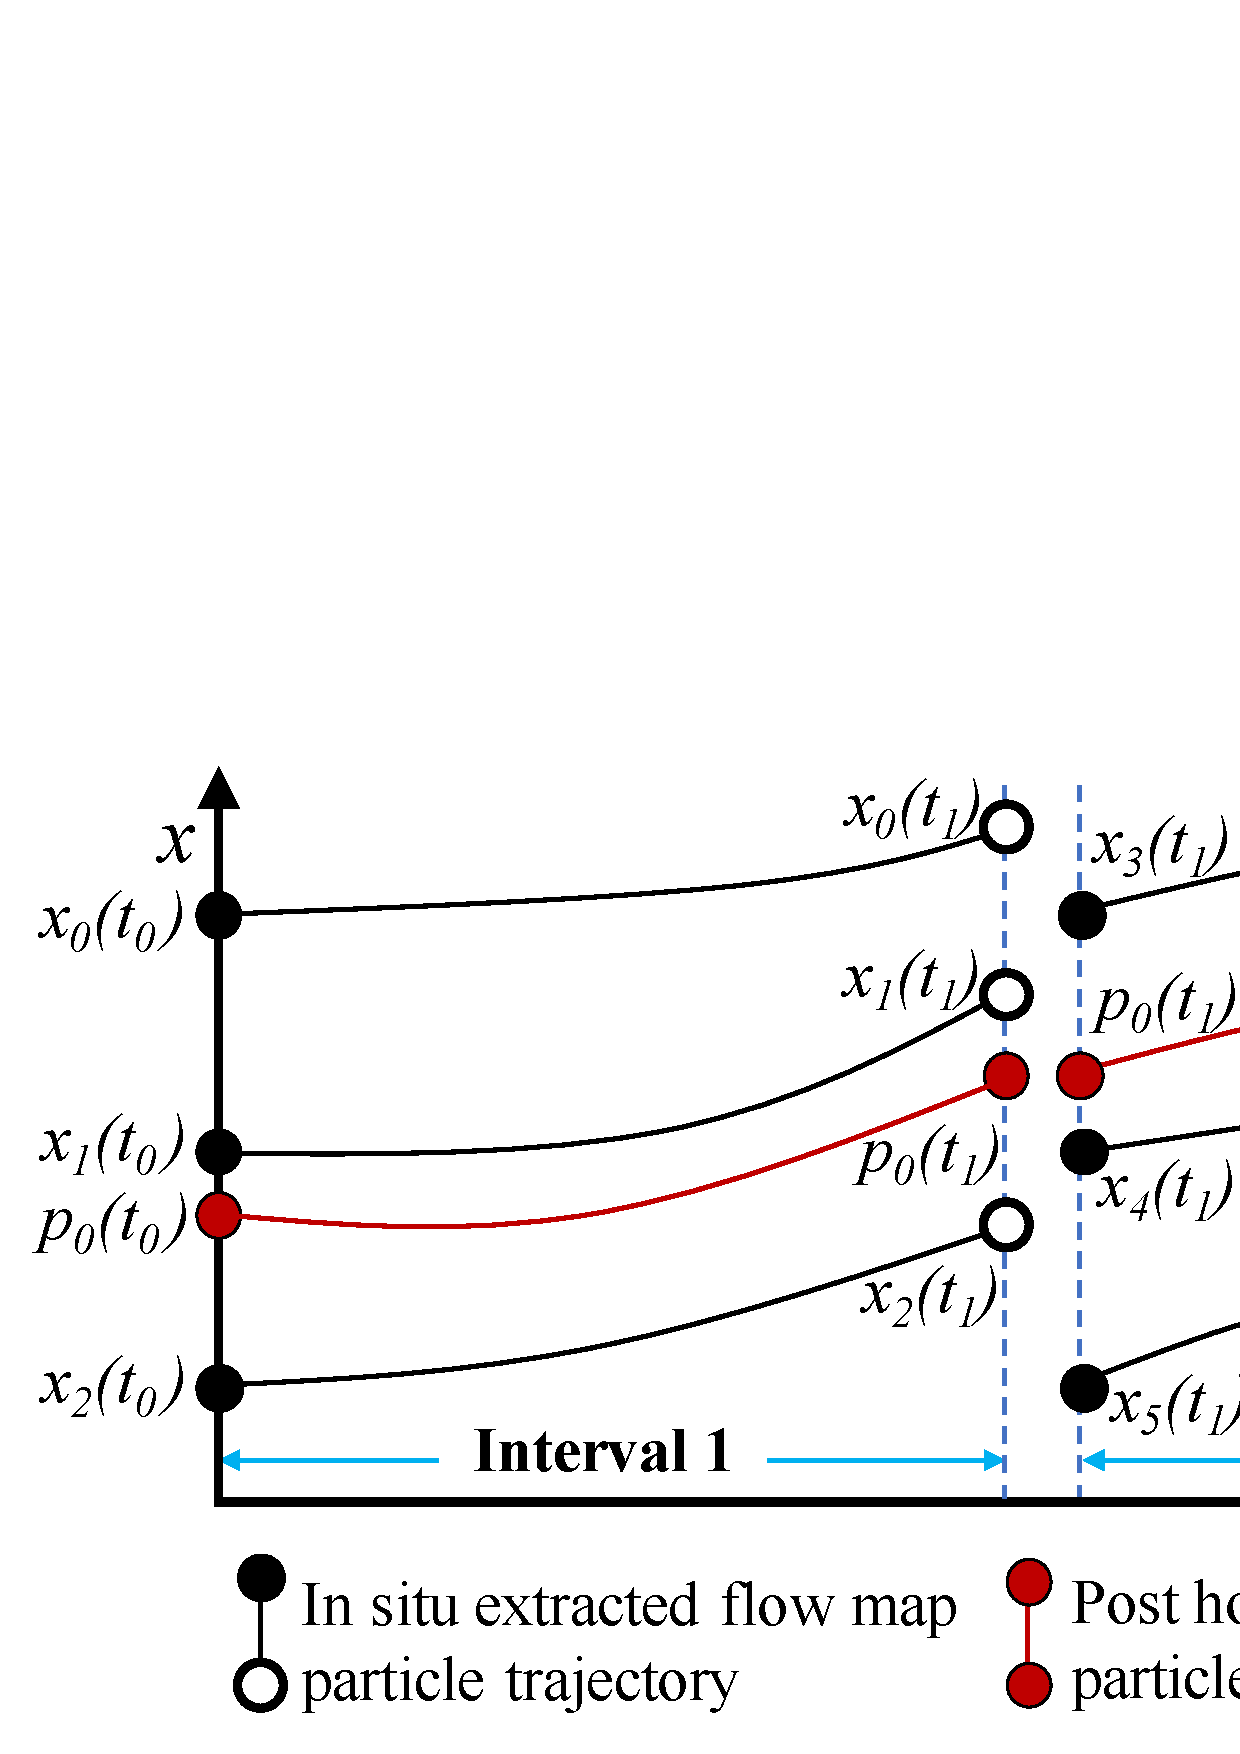
\includegraphics[width=\linewidth]{Images/phases_new_tall.pdf}
%\caption{\fix{The phases of Lagrangian analysis. The in situ phase uses uniform seed placement and extracts flow maps over temporally nonoverlapping intervals. In this example, the flow maps consist of particles \{$x_0$, $x_1$, $x_2$\} and \{$x_3$, $x_4$, $x_5$\} for the intervals [$t_0$, $t_1$] and [$t_1$,$t_2$], respectively. The flow maps are used as input during the post hoc phase. Here, the trajectory of particle $p_0$ is calculated by interpolating the flow maps over two intervals of time.}}
\caption{\fix{The phases of Lagrangian analysis. The in situ phase uses uniform seed placement and extracts flow maps over temporally nonoverlapping intervals. In this example, the flow map for the interval [$t_0$, $t_1$] consists of particles \{$x_0$, $x_1$, $x_2$\} and the flow map for the interval [$t_1$, $t_2$] consists of particles \{$x_3$, $x_4$, $x_5$\}. The extracted flow maps are used as input during the post hoc phase. Here, the trajectory of particle $p_0$ is calculated by interpolating the flow maps extracted over two intervals of time.}}
%\caption{\fix{The phases of Lagrangian analysis. The in situ phase uses uniform seed placement and extracts flow maps over temporally nonoverlapping intervals. In this example, the flow maps for [$t_0$, $t_1$] consist of \{$x_0$, $x_1$, $x_2$\} and for [$t_1$, $t_2$] consist of \{$x_3$, $x_4$, $x_5$\}. The extracted flow maps are used as input during the post hoc phase. In this example, the trajectory of particle $p_0$ is calculated by interpolating the flow maps extracted over two intervals of time.}}
\vspace{-6mm}
\label{fig:phases}
\end{figure}


Lagrangian analysis is a powerful tool to explore time-varying vector fields generated by simulations.
%
The notion of calculating a Lagrangian flow map, i.e., sets of particle trajectories, for an ocean modeling simulation ``online" for ``offline'' exploration was first proposed by Vries et al.~\cite{vries2001calculating} two decades ago.
%
More recently, compared to the traditional Eulerian technique under sparse temporal settings, Agranovsky et al.~\cite{agranovsky2014improved} evaluated reduced Lagrangian representations of time-varying vector fields and showed significantly improved accuracy-storage propositions for exploration. 
%
Figure~\ref{fig:phases} illustrates the approach.
%
The Lagrangian flow maps are computed in situ using every cycle of a simulation, i.e., the full temporal resolution.
%
After calculating and storing the flow maps, post hoc analysis tasks can use the flow maps to interpolate new particle trajectories to explore the vector field.
%
%

%
The Agranovsky et al.~\cite{agranovsky2014improved} study has been followed by several works to advance our understanding of the Lagrangian paradigm. 
%
However, the scalability of the technique while operating in situ has not been previously addressed.
%
The authors of a recent comprehensive review of Lagrangian analysis~\cite{VANSEBILLE201849}, have identified the challenges of (1) utilization of heterogenous computer architectures, (2) providing parallel performance and scalability, and (3) lack of an accessible API that allows integration with different simulations. 
%
In this paper, we address the challenge of scalability, as well as utilize a runtime in situ infrastructure for multi-physics HPC simulations and GPUs for Lagrangian flow map computation. 
%

With this study, our contributions include:
\vspace{-1mm}
\begin{itemize}[leftmargin=*,noitemsep,topsep=0pt,parsep=0pt,partopsep=0pt]
\item A scalability study of distributed-memory particle advection using GPUs for Lagrangian flow map computation. 
\item An evaluation of a proposed performance optimization, i.e., computing local Lagrangian flow maps, across multiple extraction parameter configurations.
\vspace{-1mm}
\end{itemize}

